\documentclass[aps,pra,reprint,superscriptaddress]{revtex4-1}
%\documentclass[aps,pra,reprint,groupedaddress,showpacs,showkeys]{revtex4-1}
\usepackage{amssymb}
\usepackage{amsthm}
\usepackage{amsmath} 
\usepackage{graphicx}
\usepackage{soul}
\usepackage{xcolor}
\setstcolor{red}
\usepackage[mathlines]{lineno}% Enable numbering of text and display math
%\linenumbers\relax % Commence numbering lines


\def\clau#1{\textcolor{red}{#1}}
\def\duda#1{\textcolor{green}{#1}}
\def\ale#1{\textcolor{blue}{#1}}

\begin{document}

%Title of paper
\title{The stopping power of \clau{hydrogen in} hafnium and the importance of relativistic $4f$ electrons}
%Authors and affiliations

%---------------------------Argentina
\author{C. C. Montanari}
\email{mclaudia@iafe.uba.ar}
\affiliation{Instituto de Astronom\'{\i}a y F\'{\i}sica del Espacio, 
Consejo Nacional de Investigaciones Cient\'{\i}ficas y T\'{e}cnicas - 
Universidad de Buenos Aires, Pabell\'on IAFE, 1428 Buenos Aires, 
Argentina}

%---------------------------Chile
\author{\clau{P. A. Miranda}}
\affiliation{Departamento de F\'isica, Facultad de Ciencias Naturales, 
Matem\'atica y del Medio Ambiente. Universidad Tecnol\'ogica Metropolitana. 
7800002, Chile}
%-------------------------Lisboa
\author{\clau{E. Alves}}
\affiliation{Centro de Ci\^{e}ncias e Tecnologias Nucleares, Instituto 
Superior T\'ecnico, Universidade de Lisboa, 2696-953 Sacav\'{e}m, 
Portugal}
\affiliation{Instituto de Plasma e Fus\~{a}o Nuclear, Instituto Superior 
T\'ecnico, Universidade de Lisboa, 2696-953 Sacav\'{e}m, Portugal}

%------------------------------Argentina
\author{A. M. P. Mendez}
\affiliation{Instituto de Astronom\'{\i}a y F\'{\i}sica del Espacio, 
Consejo Nacional de Investigaciones Cient\'{\i}ficas y T\'{e}cnicas - 
Universidad de Buenos Aires, Pabell\'on IAFE, 1428 Buenos Aires, 
Argentina}
%-------------------------------
\author{D. M. Mitnik}
\affiliation{Instituto de Astronom\'{\i}a y F\'{\i}sica del Espacio, 
Consejo Nacional de Investigaciones Cient\'{\i}ficas y T\'{e}cnicas - 
Universidad de Buenos Aires, Pabell\'on IAFE, 1428 Buenos Aires, 
Argentina}
%----------------------------------------------
\author{J. E. Miraglia}
\affiliation{Instituto de Astronom\'{\i}a y F\'{\i}sica del Espacio, 
Consejo Nacional de Investigaciones Cient\'{\i}ficas y T\'{e}cnicas - 
Universidad de Buenos Aires, Pabell\'on IAFE, 1428 Buenos Aires, 
Argentina}

%---------------------------- Chile
\author{R. Correa}
\affiliation{Departamento de F\'isica, Facultad de Ciencias Naturales, 
Matem\'atica y del Medio Ambiente. Universidad Tecnol\'ogica Metropolitana. 
7800002, Chile}
%----------------------------
\author{J. Wachter}
\affiliation{Departamento de F\'isica, Facultad de Ciencias Naturales, 
Matem\'atica y del Medio Ambiente. Universidad Tecnol\'ogica Metropolitana. 
7800002, Chile}
%----------------------------
\author{M. Aguilera}
\affiliation{Departamento de F\'isica, Facultad de Ciencias Naturales, 
Matem\'atica y del Medio Ambiente. Universidad Tecnol\'ogica Metropolitana. 
7800002, Chile}

%-------------------------Lisboa
\author{N. Catarino}
\affiliation{Centro de Ci\^{e}ncias e Tecnologias Nucleares, Instituto 
Superior T\'ecnico, Universidade de Lisboa, 2696-953 Sacav\'{e}m, 
Portugal}
%---------------------------
\author{R. C. da Silva}
\affiliation{Centro de Ci\^{e}ncias e Tecnologias Nucleares, Instituto 
Superior T\'ecnico, Universidade de Lisboa, 2696-953 Sacav\'{e}m, 
Portugal}

\date{\today}

%=======================================================================
%=======================================================================
\begin{abstract}
 The stopping power of protons through Hf foil has been studied both 
experimentally and theoretically. The measurements were performed at 
the Laboratory of Accelerators and X-Ray Diffraction in Lisbon, by 
using the transmission method on self-supporting stopping material. 
 The overall uncertainty of around $5\%$ was established over the 
protons energy range  (0.6-2.5) MeV. The theoretical developments 
involved fully relativistic atomic structure calculations for Hf, which 
required the solution of the Dirac equation. The shell-wise local plasma 
approximation (SLPA) was used to describe the energy transferred to the 
bound $1s$-$4f$ electrons, and the outer four electrons were considered 
as a free electron gas (FEG). We found the relativistic description of 
the $4f$-shell and the screening between $4f$ and $5p$ electrons are 
decisive around the stopping maximum. Present theoretical and 
experimental results are in very good agreement in the energy region 
of the new measurements. However, the present theoretical stopping 
cross sections show substantial differences with the most used 
semi-empirical models (SRIM2013 and ICRU-49) at intermediate to low 
energies. Our calculations suggest the stopping maximum higher and 
shifted to lower energies than these previous predictions. Future 
measurements below 100 keV would be decisive for a better knowledge 
around the maximum and below.
\end{abstract}

% insert suggested PACS numbers in braces on next line
\pacs{34.50.Bw} \keywords{Stopping power, hafnium, Relativistic atomic 
structure, Transmission method}

\maketitle

\linenumbers
%=======================================================================
%=======================================================================
\section{Introduction}
\label{intro}

For impact energies above a few keV/amu, mono-energetic charged 
particles penetrating a foil of any material lose their energy through 
a series of consecutive inelastic collisions, mainly with target 
electrons~\cite{Chu01,Sigmund}. The information given by the energy 
loss process is essential not only to have a better knowledge of the 
physics behind the fundamental interactions, but also because it plays 
an important role in many applied fields such as materials science, 
nuclear physics, ionic implantation and radiotherapy~\cite{Sigmund,Schardt}. 
Experimental data on ion mean energy loss per unit path $S(E)$ is of 
crucial relevance to check the reliability of semi-empirical models and 
to determine some key parameters~\cite{Diwan,Damache04,Damache02}. The 
experimental data available is often rather scarce, which is troublesome 
when the material under study corresponds to an element of low 
occurrence on the Earth's upper crust, such as hafnium.

So far, only one experimental work has been published regarding the 
stopping power cross section of pure hafnium for protons~\cite{Sirotinin}, 
while more attention has been recently given to  studies involving 
hafnium oxide due to its practical use~\ale{\cite{Abril,Behar,Primetzhofer,Roth}}. 
It is well known that significant attention has been paid in recent 
years to transition metal-oxides such as HfO$_2$ because of their 
potential as alternative gate dielectrics to replace SiO$_2$ for the 
future generation of nano-electronics with less than 45 nm gate 
length~\cite{Choi,Robertson}. Some important physical properties of the 
above mentioned metal-oxide films depend on its thickness, which is 
often measured by using Rutherford Backscattering Spectrometry~\cite{Alfassi01,Tesmer01}, 
a method that relies heavily on the determination of the stopping power 
of ion beams in the material of interest.

In this study, we report experimental stopping power cross sections 
over the incident energy range (0.6-2.5) MeV for protons crossing 
self-supported Hf thin-film by using the transmission method. We aim 
not only to upgrade stopping power data compilations~\cite{HPaul03,mondim17} 
but also to provide useful information about the processes governing 
the slowing down of protons in multi-electronic targets. In the rare 
earth metals, the $4f$ electrons play a relevant role in the stopping 
power, being the first shell of bound electrons below the conduction 
band. As already noted \cite{Roth17}, the free electron gas (FEG) shows 
unexpected behavior in these elements, which casts doubts on its proper 
description. In the case of Hf, we found the contribution of the 
$4f$-shell decisive even at impact energies around the stopping maximum, 
as shown later.

The theoretical approach implemented in this work uses the shell-wise local plasma approximation (SLPA)~\cite{mon13} to describe the energy 
transferred to the bound $1s$-$4f$ electrons, and two different models 
for the FEG: \clau{in low energy region,}
the screened potential with cusp condition model (SPCC)~\cite{mon17}, 
which is non-linear binary formalism; and the Mermin-Lindhard dielectric 
formalism (ML)~\cite{Mermin}, for energies around the stopping maximum 
and above. Our model requires the relativistic wave functions and 
binding energies of Hf, and considers 4 electrons per atom in the 
FEG~\cite{mendez2019}. Hf has the extra interest of the filled 
$4f$-subshell (with 14 electrons) as the main contribution below the 
FEG, causing the stopping cross sections to be very sensitive to a good 
description of this shell. The screening among the $4f$ and $5p$ 
electrons has been considered and found to play a major role within the 
SLPA calculations.

The experimental details and data are given in Section~\ref{experiment}, 
while the theoretical method is explained in Section~\ref{theory}. 
Present theoretical and experimental values are finally compared to the \clau{only experimental values by Sirotinin group~\cite{Sirotinin} measured with backscattering method, the theoretical results by  Grande and Schiwietz~\cite{Grande,casp52}, and by Sigmund and Schinner~\cite{DPASS20}, and also with the semi-empirical values from the SRIM-2013 package~\cite{Ziegler01} and the ICRU-49 tabulation~\cite{ICRU49}}. 
Conclusions and discussions are given in Section~\ref{conclusion}. All 
the present data can be found at the Zenodo platform \cite{zenodo}.

%-----------------------------------------------------------------------
\begin{figure}[!t]
\centering
\includegraphics[width=9cm]{Fig01.eps}
\caption{RBS spectrum for $E_{\mathrm{avg}}=921.1$ keV protons on 
hafnium sample which is subsequently used to determine the energy loss 
in the foil.}
\label{F01}
\end{figure}


%=======================================================================
\section{EXPERIMENTAL ARRANGEMENTS}
\label{experiment}

%-----------------------------------------------------------------------
\subsection{Accelerator and scattering Chamber}
The procedure used in this work to obtain stopping power data is 
essentially the same as described in Ref.~\cite{Miranda01}. The present 
measurements were made at the IST/LATR (Laboratory of Accelerators and 
X-Ray Diffraction) in Lisbon. This facility uses a 2.5 MV Van de Graaff 
accelerator to deliver $^1$H$^+$ primary ion beams through a series of 
electrostatic lenses and collimators onto a thin Au/SiO$_2$ sample which 
is used as a scattering center. This sample was placed in the center of 
a RBS/C scattering chamber, where a high vacuum (pressure of 
$\sim$10$^{-6}$ Torr) was maintained during the measurements. The beam 
current on the sample was kept at around 5.0 nA to attain sufficient 
statistics in each particle spectrum. By using a beam spot of about 
1.0 mm in diameter, a solid angle of 11.4 msr was attained. The overall 
energy resolution (FWHM) of the detection system was about 15 keV 
relative to 5.486 MeV alpha particles from a $^{241}$Am source.

%-----------------------------------------------------------------------
\subsection{Target}
The stopping material under analysis was a hafnium foil with nominal 
thickness of 1.0 $\mu$m and 99.95\% purity which was supplied by Lebow 
Company~\cite{Lebow}. However, a more precise thickness value was 
achieved by measuring the energy loss of alpha particles coming from a 
calibrated ($^{239}$Pu, $^{241}$Am, $^{244}$Cm) source. From the alpha 
spectra with and without the Hf foil interposed, the characteristic 
energy shift $\delta$E was measured and then combined with the stopping 
power for 5.486 MeV alphas on hafnium (55.69 eV/$10^{15}$ at/cm$^2$) 
found in Ref.~\cite{Ziegler01} to obtain an areal density of 
($4.13 \pm 0.21$)$\times 10^{19}$ at/cm$^2$ which corresponds to a 
thickness of $0.920\pm0.046 \mu$m.

%-----------------------------------------------------------------------
\subsection{Energy loss measurement}
Once the beam impinges on the Au/SiO$_2$ sample, protons are 
back-scattered towards a Si surface barrier detector located at 
140$^{\circ}$ relative to the initial beam direction. Fig.~\ref{F01} 
shows two particle spectra where ion energies $E_2$ and $E_1$ are 
associated to a placed and removed hafnium sample, respectively. Both 
energy distributions were fitted by Gaussian functions to obtain the 
mean energy and width (FWHM) of the peaks \cite{Sun01}, and from the 
difference between these two peak positions in the spectrum, the total 
energy loss $\Delta E = (E_1 - E_2)$ in the foil was calculated. As 
established in previous studies \cite{Miranda01,Damache02}, the 
experimental stopping power cross sections $\varepsilon (E) $ are 
determined at some mean energy $E_{\mathrm{avg}}$ by measuring the ion 
energy losses $\Delta E$ within the investigated Hf foil, which has a 
mean thickness denoted by $\Delta x$. In this way, only when the energy 
loss fraction $\Delta E/E_{\mathrm{avg}}$ across the Hf foil is not 
exceeding 20\% it is possible to define the stopping cross section by 
\cite{Raisanen01,Schulz01}:
\begin{equation}\label{eq:stcross}
 \varepsilon(E)=\frac{S(E)}{N}=-\frac{dE}{N\,dx}\approx-\frac{\Delta E}{N\Delta x},
\end{equation}
where $N$ denotes the atomic number density (atoms cm$^{-3}$) of the 
material under study. When this condition was not fulfilled, a small 
correction to the mean energies $E_{\mathrm{avg}}$ was applied in order 
to account for the nonlinear dependence on ion energy of stopping 
powers \cite{Chilton,Rajatora}.


%=======================================================================
\section{Theoretical Method} 
\label{theory}
The energy loss of ions in metal targets responds to different physical 
mechanisms, depending on the impact ion velocity. At low velocities, the 
binary collisions are responsible for the loss of energy by the ion. 
The main contribution is the ionization of electrons of the metal 
conduction band, which is well approximated by a free electron gas (FEG) 
of Fermi velocity $v_F$. Above certain velocity (i.e. $v\geq 1.5\,v_F$), 
not only binary but also collective excitations (plasmons) 
\ale{occur}~\cite{mon17}. Moreover, at high energies, also the bound electrons 
contribute to the stopping power. The method used in this work combines 
a description for the interaction with the valence (or conduction) 
electrons as a FEG, and a different one for the interaction with the 
bound electrons.

We used the SPCC model~\cite{mon17} to describe the stopping power of 
low velocity charged particles in the FEG. It is a non-perturbative 
binary collisional approximation, thus valid at energies below that of 
plasmon excitations.  The SPCC~\cite{mon17} is based on a screened 
central potential with cusp condition of the electronic density close 
to the projectile. This model proved to give a good description of the 
induced electron density even for negative projectiles~\cite{mon17}, 
and reproduces the low velocity proton-antiproton differences in the 
stopping power (Barkas effect). The SPCC formalism only depends on the 
Wigner-Seitz radio, $r_S$, which is a measure of the electronic density 
of the FEG. For metals of well-known $r_S$, the SPCC describes correctly 
the low energy experimental stopping data~\cite{mon17}, agreeing with 
the DFT results by Echenique and coworkers~\cite{eche81,nagy89} at $v=0$. 

Hafnium ($Z=72$, [Xe] $4f^{14}\,6s^2\,5d_{3/2}^1\,5d_{5/2}^1$), belongs 
to the first groups of transition metals, with \ale{four} electrons as FEG 
(\st{theoretical} $r_S=2.14$ a.u.) and $1s$-$4f$ electrons bound. We compared 
the computed $r_S$ with the experimental value obtained from measured 
energy loss function by Lynch \textit{et al} \cite{lynch75}. The 
experimental plasmon energy of Hf is $\hbar\omega_P \approx 15.8$ eV, 
with a width at half maximum $\delta \approx 4.4$ eV, and 
$r_S \approx 2.07$ a.u. \cite{lynch75}. The difference of less than 
$5\%$ between theoretical and experimental $r_S$ assess Hf as a 
canonical target~\cite{mon17}.

Above certain impact velocity, the plasmon contribution is important 
(i.e. around and above the stopping maximum). An interesting value for 
our analysis is the minimum impact velocity to excite plasmons, $v_P$. 
In the dielectric formalism, this value can be obtained as 
$v_P\,\approx\,v_F[1+(3\pi\,v_F)^{-1/2}]$~\cite{suppression}. To 
describe the energy loss considering collective and binary excitation, 
we resort to the ML dielectric formalism \cite{Mermin}, which is a 
linear response, perturbative approximation, so it depends on the 
square of the ion charge. In this formalism, the response of target 
electrons to the ion passage is described through the quantum dielectric 
function, depending on the characteristic $r_S$ and $\delta$ parameters 
of the FEG. 

%----------------------------------------------------------------------
\begin{figure*}[!t]
\centering
\includegraphics[width=11.cm]{bindener.eps}
\caption{(a) Binding energies of Hf. \clau{Present relativistic and available non-relativistic~\cite{badnell97}  
values} are given with filled symbols. Experimental measurements 
for solids~\cite{williams1995} are depicted with open circles. 
(b) Corresponding relative errors respect to experimental data.}
\label{Binding_E}
\end{figure*}
%------------------------------------------------------------------------

For the stopping power due to bound electrons, the SLPA~\cite{mon17,mon13} 
is employed. It is worth \ale{mentioning} that the only inputs for the SLPA 
are the space-dependent densities of each shell in the ground state, 
and their binding energies. Collective processes and screening among 
electrons are included. \ale{Since} hafnium is a relativistic target, the 
wave functions and binding energies must be obtained by solving the 
\ale{many-electron} Dirac Hamiltonian. Details of these calculations 
\clau{and a table of binding energies} have been published in 
Ref.~\cite{mendez2019}, while Slater-type orbital expansions are 
given in \cite{Hf_arxiv}.

\ale{To} assess the importance of  \clau{a full relativistic} description of 
bound electrons, Fig.~\ref{Binding_E} (a) shows our \st{relativistic} binding 
energies, $E_{nl\pm}$, with $\pm=j\pm1/2$; the 
non-relativistic values~\cite{badnell97}; \clau{and the experimental data on 
solid Hf~\cite{williams1995}, which is available only for $1s$ to $4f_{\pm}$ 
subshells, as expected.} 
We notice that not only the most inner shells require relativistic calculations, but also the outer $5p$ and $4f$ shells. Furthermore, this figure shows very clearly the disability of non-relativistic calculations to describe the experimental data, which surprisingly worsens from the inner to the outer shells.

\clau{In the comparison with the experimental values in Fig.~\ref{Binding_E} (a) it can be noted that}
\ale{\st{Also,} the sign of the binding energy deviations is inverted}  \clau{for the outer $5s$-$4f\pm$ electrons, with the experimental binding energies being less bounded than our theoretical ones. Small differences for the outer shells are expected since } 
\ale{\st{can be attributed to the fact that} the experimental
values correspond to hafnium in solid-state, while our theoretical  calculations correspond to the element in the gas phase.}
%i.e. the electrons go from being more bounded --than the experimental values-- to being less bounded.

\clau{For more detail, Fig.~\ref{Binding_E} (b) shows}  the relative errors %\clau{of theoretical (relativistic and non relativistic)} 
with respect to the experimental  values. %\ale{\st{The relativistic binding energies of the electrons belonging to the deep K, L and M shells deviate less than $2.5\%$ from the experimental values, while the non-relativistic ones are within $\sim10\%$. Moreover, we notice that the relativistic corrections greatly influences the outer shells. This effect may be consequence of the orthogonality with the relativistic inner shells.}}
%\clau{ \st{This figure shows clearly that the relativistic corrections are decisive to describe the outer shells. The solution of the Dirac equation from inner to outer shells, and the orthogonality of the wave functions, involves all the shells.  }} 
\duda{This figure shows clearly that \st{for this target,} the relativistic corrections are very important to describe
the atomic structure of hafnium, even for the outer shells.
It turns out that the errors committed in the non-relativistic calculations of the inner shell orbitals 
propagate, through the Hartree-Fock approximation, to the outer shells.} \clau{The importance of full-relativistic calculations for the outer shells has already been noted for Au, Pb and Bi and W~\cite{mon09}.}


\clau{For the contribution of bound electrons to the total stopping cross sections}, the SLPA considers independent contributions of each subshell. Our relativistic binding energies present spin-orbit split. However, in total stopping power, where the initial state of the excited electron is not measured, the quantum uncertainty in energy $\Delta E$ melts this split. The criteria $\Delta E\Delta t\geq\hbar/2$ merges the energies 
$E_{nl+}-E_{nl-}$ for sufficiently small values of $\Delta t$ (the 
collisional mean-time). In fact, at sufficiently high impact velocity, 
we can expect all target electrons to respond together to the ion 
passage~\cite{lindhard53,chu72}. Following previous works~\cite{mon09},
the collisional time is estimated as $\Delta t\approx\langle r_i\rangle/v$, 
with $\langle r_i\rangle$ and $v$ being the orbital mean radio and 
impact velocity, respectively. 
\clau{In the case of hafnium}, we found that for every sub-shell of electrons, the spin-orbit split is unresolved in the energy region this sub-shell contributes. Therefore, the $nl$-electrons should be 
considered together, responding to the ion passage as a single gas of 
electrons with density $\delta_{nl}(r)$ and a mean binding energy 
$E_{nl}$. This feature is important within the SLPA calculations because 
it accounts for the screening among electrons of the \textit{same} 
binding energy. For example, the $4f_{-}$ and $4f_{+}$ of Hf can only 
be resolved for impact energies $E<0.05$ keV, but the contribution of 
$4f$ to the total stopping is negligible for $E<40$ keV. Moreover, the 
$5p$ and $4f$ electrons of Hf are very close in energy 
($\Delta E_{5p-4f} \approx 1$ a.u.~\cite{mendez2019}) and they react 
together for impact energies $E>40$ keV (inter-shell screening). \clau{As already mentioned, at higher energies inter-shell screening is possible for other subshells (i.e. 4p-4d for impact energies above 0.9 MeV), but its weight in the total stopping is minor for deeper shells.}

%-----------------------------------------------------------------------
\begin{figure*}[!t]
\centering
\includegraphics[width=13.cm]{Fig02_new3.eps}
\caption{(colour online) Theoretical stopping cross sections of protons in hafnium. \clau{Blue dash-dotted-line,the non-perturbative SPCC for the FEG; blue solid-line, ML results for the FEG (includes plasmon excitation); red
solid and dotted-lines, the SLPA results for bound electrons with and without $5p$-$4f$ screening, respectively. Black curves, total  stopping
adding the FEG and bound $1s$-$4f$ contributions: dash-dotted-line, SPCC (FEG) + SLPA (bound); solid-line, ML (FEG) + SLPA (bound) with 4f-5p screening; dotted-line, ML (FEG) + SLPA (bound) without 4f-5p screening.}
The vertical grey dashed-line indicates the energy \clau{of 37 keV} above which plasmon 
excitation is possible.} 
\label{slpa4f}
\end{figure*}
%-----------------------------------------------------------------------


\clau{Finally, in all our calculations~\cite{mon17} we assumed the projectile to be proton and not neutral hydrogen. When an ion moves inside a metal, the FEG screens the nucleus, so the binding energies will be smaller than outside the metal, and this effect is more important a low impact velocities $v$. In the case of hydrogen the difference is drastic, i.e. for H inside Hf ($rs=2.07$), the $1s$-bound state is almost null at $v<2$~\cite{suppression}. It is worth to mention that this assumption agrees with Ziegler SRIM code~\cite{Ziegler01}, but differs from CasP code~\cite{Grande} that predicts neutral hydrogen at very low velocities \st{based on measurements of charge states outside the metal}.}

%-----------------------------------------------------------------------
\begin{figure*}[!t]
\centering
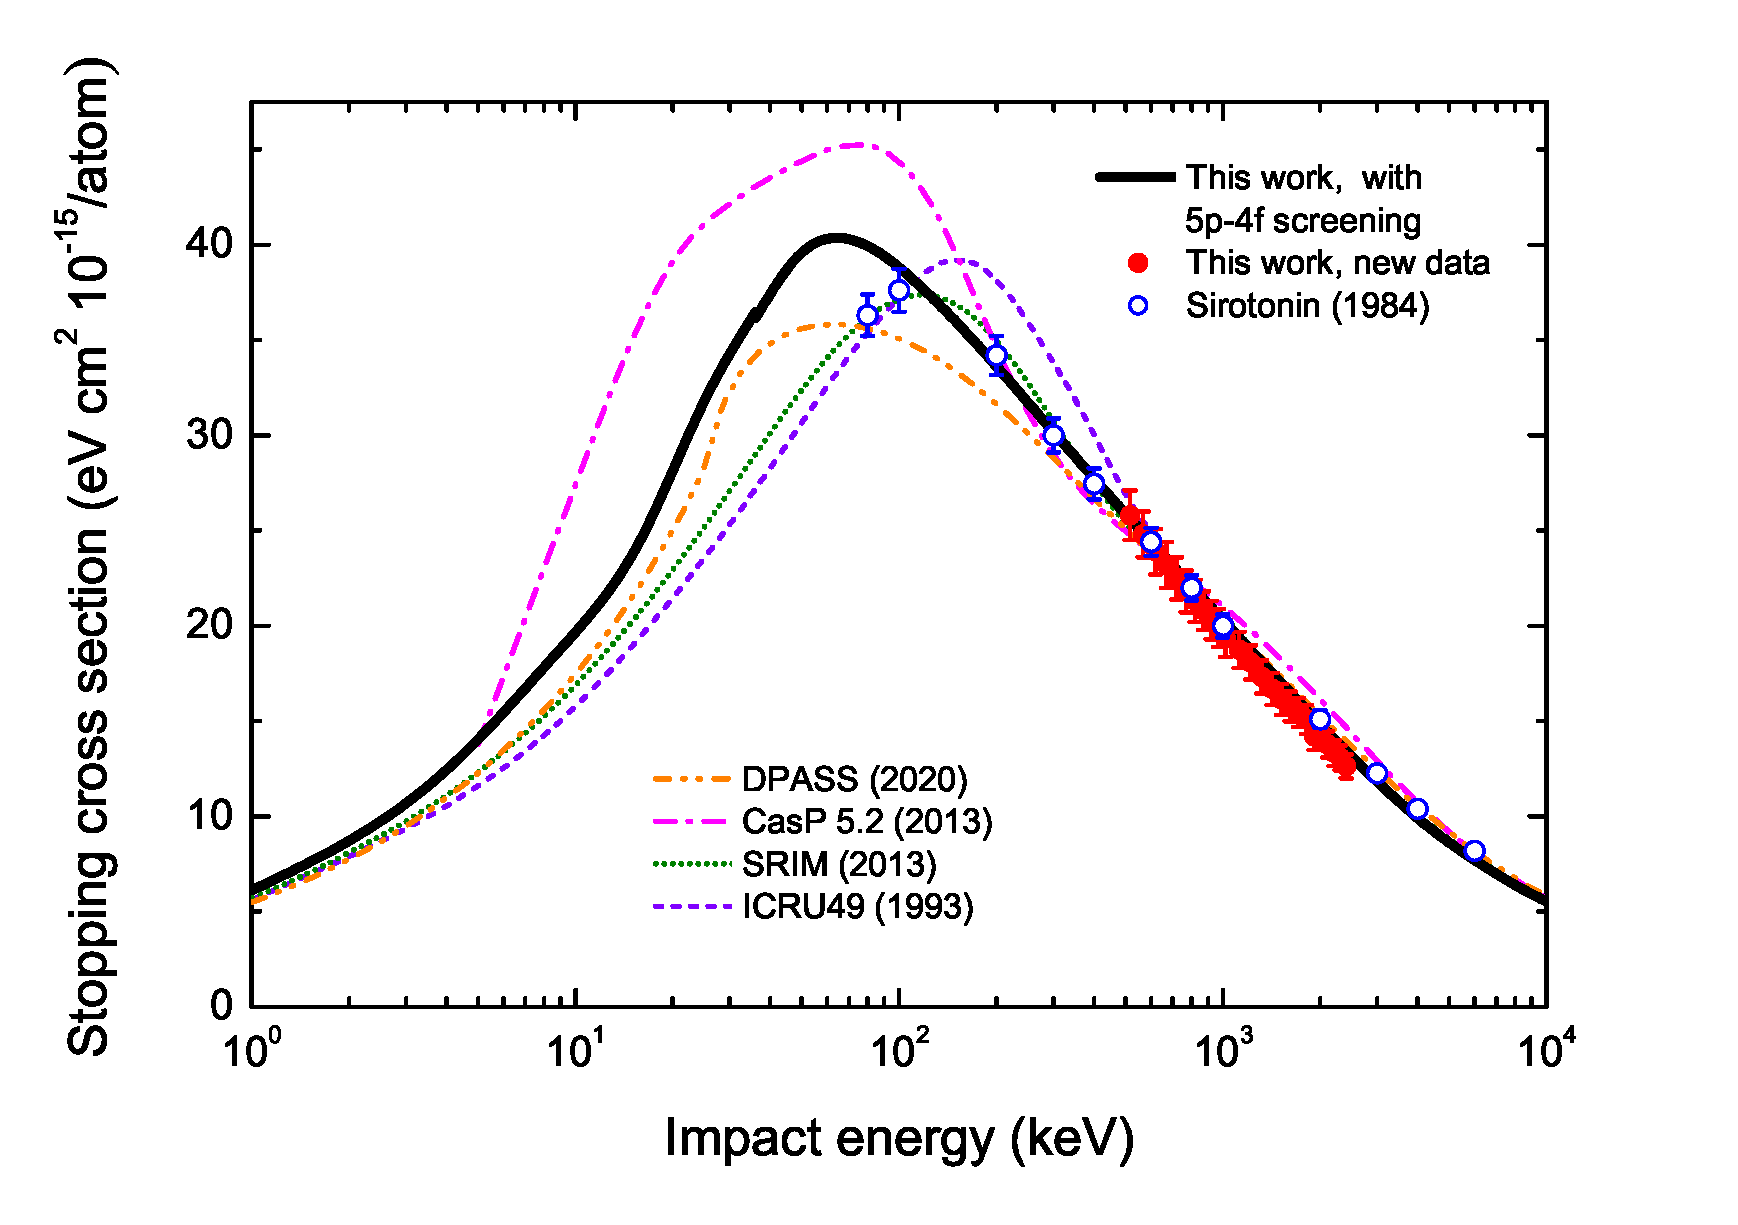
\includegraphics[width=13.0cm]{Fig03_new2.eps}
\caption{(colour online) Stopping power cross section of hafnium for protons. Symbols: 
solid circles, present values; open circles, previous data~\cite{Sirotinin}. 
Curves: Black solid-line, present full theoretical results with 
$4f$-$5p$ screening; \clau{pink dash-dot line, theoretical CasP5.2~\cite{Grande,casp52} values; orange dash-double-dot line, theoretical DPASS~\cite{DPASS20} results; } green dotted-line, semi-empirical SRIM-2013~\cite{Ziegler01}; violet dashed-line, ICRU49~\cite{ICRU49} tabulated values.}
\label{F03}
\end{figure*}
%-----------------------------------------------------------------------

In Fig.~\ref{slpa4f}, we display the present theoretical stopping cross
section of Hf for protons \clau{using the relativistic wave functions and binding energies, but} with and without the $5p$-$4f$ screening. \clau{We show separately the FEG and bound electron contributions and the total stopping as the addition of both of them.}
\st{added the FEG and the bound electron contributions as explained above. }
The minimum energy for plasmon excitation was estimated $\sim 37$ keV. We
used the non-perturbative SPCC model for impact energies $E \leq 37$~keV, 
and the perturbative ML calculation above this energy. \clau{Bound $1s$-$4f$ electrons (relativistic wave functions and binding energies) are calculated with the SLPA and shown separately in Fig.~\ref{slpa4f} with and without the $4f$-$5p$ screening. Below $\sim 40$ keV the difference between both calculations is negligible}. Clearly, 
considering $5p$-$4f$ electrons as a single group of 20 electrons with 
screening among them gives lower stopping values than the addition of 
the separate $5p$ and $4f$ contributions. Notice that this shell 
correction can \st{only} be considered \duda{self-consistently? naturally? intrinsically?} within a many electron model such as the SLPA, .

%=======================================================================
\section{Analysis of the results and discussion}
\label{discussion}

The present data \st{and theoretical results are} is displayed in 
Table~\ref{table01}. %, and Fig.~\ref{F03}. 
As can be \clau{observed,} %seen in Table~\ref{table01},
an overall relative uncertainty of around 5\% was 
achieved for the experimental stopping power values, which are mainly 
due to the uncertainty in the hafnium foil thickness. 

%-----------------------------------------------------------------------
\begin{table*}[!t]
\centering
\caption{Stopping power values S$_{\mathrm{exp}}$ of hafnium for protons measured 
in this work. $\Delta$E/E values are also shown.}
\label{table01}

\vspace{0.2cm}

\begin{ruledtabular}
\begin{tabular}{ccc|ccc|ccc} %\hline\hline
E$_{\mathrm{avg}}$ & S$_{\mathrm{exp}}$       & $\Delta$E/E & E$_{\mathrm{avg}}$ & S$_{\mathrm{exp}}$       & $\Delta$E/E & E$_{\mathrm{avg}}$ & S$_{\mathrm{exp}}$       & $\Delta$E/E \\
keV                & eV/(10$^{15}$ at/cm$^2$) & \%          & keV                & eV/(10$^{15}$ at/cm$^2$)	& \%          & keV                & eV/(10$^{15}$ at/cm$^2$) & \% \\ \hline
516.6	 & 25.8	$\pm$	1.3	&	20.5	&	1170.3	&	18.25	$\pm$	0.91	&	6.4	&	1813.4	&	15.10	$\pm$	0.76	&	3.4	\\
567.8	 & 24.8	$\pm$	1.2	&	17.9	&	1220.0	&	18.08	$\pm$	0.90	&	6.1	&	1862.7	&	14.79	$\pm$	0.74	&	3.3	\\
618.8	 & 23.9	$\pm$	1.2	&	15.8	&	1269.6	&	17.57	$\pm$	0.88	&	5.7	&	1912.0	&	14.21	$\pm$	0.71	&	3.0	\\
669.6	 & 23.2	$\pm$	1.2	&	14.2	&	1319.2	&	17.32	$\pm$	0.87	&	5.4	&	1961.2	&	14.46	$\pm$	0.72	&	3.0	\\
720.1	 & 22.5	$\pm$	1.1	&	12.8	&	1368.8	&	17.15	$\pm$	0.86	&	5.1	&	2010.4	&	14.34	$\pm$	0.72	&	2.9	\\
770.5	 & 21.8	$\pm$	1.1	&	11.6	&	1418.3	&	16.69	$\pm$	0.83	&	4.8	&	2059.6	&	13.76	$\pm$	0.69	&	2.7	\\
820.8	 & 21.3	$\pm$	1.1	&	10.7	&	1467.8	&	16.43	$\pm$	0.82	&	4.6	&	2108.8	&	13.78	$\pm$	0.69	&	2.7	\\
871.0	 & 20.8	$\pm$	1.0	&	9.8	&	1517.2	&	16.13	$\pm$	0.81	&	4.4	&	2158.0	&	13.70	$\pm$	0.69	&	2.6	\\
921.1	 & 20.3	$\pm$	1.0	&	9.1	&	1566.7	&	16.04	$\pm$	0.80	&	4.2	&	2206.5	&	13.33	$\pm$	0.67	&	2.5	\\
971.1	 & 19.9	$\pm$	1.0	&	8.4	&	1616.0	&	15.77	$\pm$	0.79	&	4.0	&	2256.4	&	13.27	$\pm$	0.66	&	2.4	\\
1021.0 & 19.33	$\pm$	0.97	&	7.8	&	1665.4	&	15.51	$\pm$	0.78	&	3.8	&	2305.5	&	13.07	$\pm$	0.65	&	2.3	\\
1070.8 & 19.03	$\pm$	0.95	&	7.3	&	1714.8	&	15.46	$\pm$	0.77	&	3.7	&	2354.7	&	12.91	$\pm$	0.65	&	2.2	\\
1120.6 & 18.73	$\pm$	0.94	&	6.9	&	1764.1	&	14.93	$\pm$	0.75	&	3.5	&	2403.8	&	12.61	$\pm$	0.63	&	2.2	\\ \\ 
\end{tabular}
\end{ruledtabular}
\end{table*}

Fig.~\ref{F03} \clau{synthesizes the results of the present work.} \st{, we have good} \clau{The} agreement between the present 
theoretical results and the \clau{new} measurements displayed in Table~\ref{table01} \clau{is clear}. \clau{Present measurements using transmission method are in good agreement with the previous data by 
Sirotinin~\cite{Sirotinin}, measured in backscattering geometry}. Our theoretical approach also agrees with the data by 
Sirotinin~\cite{Sirotinin}, except for the lowest energy measurement at 
80 keV. \clau{We have also included in this figure the theoretical curves from Grande and Schiwietz CasP5.2 code~\cite{Grande,casp52} and from Sigmund and Schinner DPASS code~\cite{DPASS20}, both available online; also the semi-empirical results from SRIM-2013~\cite{Ziegler01} and the ICRU49 tables~\cite{ICRU49}}. It is interesting that our full theoretical curve differs from 
SRIM-2013 for impact energies below 100 keV. We obtain a stopping 
maximum around $40 \times 10^{-15}$ eV cm$^2$/atom  at 65 keV. Instead,
following the up-to-now only set of data \cite{Sirotinin}, SRIM-2013
suggests a lower stopping maximum  at impact energy of 115 kev. 
\clau{The stopping maximum is a very sensitive region for any full theoretical description, with no parameters at all, and this is quite visible in a linear-scale plot like Fig.~\ref{F03}. However, the impact energy for the maximum seem to agree between our curve and DPASS, although is $10 \%$ below. Instead, CasP predicts a stopping maximum $10 \%$ above our value and a completely different shape at lower energies.}
It is 
worth mentioning that \clau{our model gives} similar \st{theoretical} results using the experimental 
$r_S=2.07$ a.u. instead of the theoretical $r_S=2.14$ a.u. \st{give} \clau{with} the 
stopping maximum at the same impact energy but $4\%$ higher. 

Future experiments \st{for impact energies below 100 keV} would be important to
complete this study \clau{on the stopping of Hf for protons. In the energy region $80-500$ keV only the measurements by Sirotinin group~\cite{Sirotinin} in 1984 are available. SRIM-2013 clearly includes these values in the adjust of the code, so it does not represent a test for this data. Undoubtedly, new measurements are needed in three specific energy regions: below 500 keV, around the stopping maximum (i.e. $50-200$ keV) and at low impact energies. } 

%=======================================================================
\section{Conclusion}
\label{conclusion}

In this work, we have used the transmission method to experimentally 
determine stopping power cross section values for (0.6-2.5) MeV protons 
incident on self-supporting Hf foils with an overall uncertainty of 
around 5\%. Additionally, we calculated values extracted from the 
theoretical framework that involved the relativistic wave functions and 
binding energies of Hf, and considered four electrons per atom in the free 
electron gas. The shell-wise local plasma approximation was employed to 
describe the energy transferred to the bound $1s$-$4f$ electrons, and 
two different models for the FEG: the screened potential with cusp 
condition (SPCC model) for energies below that of the plasmon 
excitation, and the Mermin-Lindhard dielectric formalism, for energies 
around the stopping maximum and above. Present theoretical stopping 
cross sections cover an extensive energy range from 1 keV/amu-10 MeV/amu.

At high impact energies, the new stopping  measurements are in good 
agreement with our theoretical results, with previous experimental data
and semi-empirical values by SRIM-2013 and ICRU-49.  However, we call 
the attention that around the stopping maximum and at lower impact 
energies the difference between our full-theoretical results and SRIM 
is substantial. \clau{We compare our theoretical results with other two models given by the DPASS and CasP5.2 codes. Differences can be noted at intermediate to low impact energies, but  they also support an stopping maximum at lower energy than SRIM predictions}. 

To the best of our knowledge, these are the first 
theoretical calculations of stopping in Hf taking into account the 
atomic relativistic effect \clau{and the screening among electrons in a consistent way from very low to high impact energies}. Future experiments for impact energies 
\clau{around the stopping maximum and in the low energy region} would be important to \st{complete  this study} \clau{have a more complete knowledge of the stopping of protons in hafnium}.

%=======================================================================
\begin{acknowledgments}
This work was funded by VRAC Grant Number L1-17 of Universidad 
Tecnol\'ogica Metropolitana, Chile; also by the Consejo Nacional de 
Investigaciones Cient\'ificas y T\'ecnicas (CONICET), the Agencia 
Nacional de Promoci\'on Cient\'ifica y Tecnol\'ogica (ANPCyT), and 
Universidad de Buenos Aires (UBA), from Argentina.

The authors gratefully acknowledge the invaluable contribution of F. 
Baptista from ITN/IST-UTL, Sacav\'{e}m, Portugal for his constant 
availability. 
\end{acknowledgments}
%=======================================================================
%  references
\begin{thebibliography}{00}
%=======================================================================
%Fundamentals of Stopping Power and Energy Loss processes
\bibitem{Chu01} 
W.K. Chu, J.W. Mayer, and M.A. Nicolet,
\textit{Backscattering Spectrometry}
(Academic Press, New York, 1978).

\bibitem{Sigmund} 
P. Sigmund, 
\textit{Particle Penetration and Radiation Effects. General Aspects and 
Stopping of Swift Point Charges}.
(Springer Series in Solid-State Sciences, Springer, Berlin, 2006), Vol. 151.

\bibitem{Schardt} 
D. Schardt, T. Els\"asser, D. Schulz-Ertner, 
Rev. Mod. Phys. \textbf{82},  383-425 (2010).

\bibitem{Diwan} 
P.K. Diwan, S. Kumar, 
Nucl. Instr. and Meth. B \textbf{359}, 78-84 (2015).

\bibitem{Damache02} 
D. Moussa, S. Damache and S. Ouichaoui, 
Nucl. Instr. and Meth. B \textbf{268}, 1754-1758 (2010); 
\textbf{343},  44-47 (2015).

\bibitem{Damache04} 
S. Damache, S. Ouichaoui, A. Belhout, A. Medouni and I. Toumert, 
Nucl. Instr. and Meth. B \textbf{225}, 449-463 (2004).

%=======================================================================
%% Use of Hafnium and Stopping Power of Hafnium
\bibitem{Sirotinin} 
E.I. Sirotinin, A.F. Tulinov, V.A. Khodyrev, V.N. Mizgulin, 
Nucl. Instr. and Meth. B \textbf{4}, 337-345 (1984).

\bibitem{Abril} 
I. Abril, M. Behar, R. Garcia Molina, R.C. Fadanelli, L.C.C.M. Nagamine, 
P.L. Grande, L. Sch\"unemann, C.D. Denton, N.R. Arista, E.B. Saitovich,
Eur. Phys. J. D \text{54}, 65-70 (2009).

\bibitem{Behar} 
M. Behar, R.C. Fadanelli, I. Abril, R. Garcia-Molina, C.D. Denton, 
L.C.C.M. Nagamine, N.R. Arista, 
Phys. Rev. A \textbf{80},  062901 (2009).

\bibitem{Primetzhofer} 
D. Primetzhofer, 
Nucl. Instr. and Meth. B \textbf{320}, 100-103 (2014).

\bibitem{Roth}
\ale{D. Roth, B. Bruckner, G. Undeutsch, V. Paneta, A. I. Mardare, 
C. L. McGahan, M. Dosmailov, J. I. Juaristi, M. Alducin, 
J. D. Pedarnig, R. F. Haglund, Jr., D. Primetzhofer, and P. Bauer
Phys. Rev. Lett. \textbf{119}, 163401 (2017).}

%=======================================================================
% Why Hafnium is so important:
\bibitem{Choi} 
J.H. Choi, Y. Mao, J.P. Chang, 
Mat. Sci. Eng. R \textbf{72}, 97-136 (2011).

\bibitem{Robertson} 
J. Robertson, R.M. Wallace, 
Mat. Sci. Eng. R \textbf{88}, 1-41 (2015).

%=======================================================================
%Importance of Stopping Power for Ion Beam Analysis
\bibitem{Alfassi01} 
Z.B. Alfassi,
\textit{Non-destructive elemental analysis}
(Blackwell Publishing, Oxford, 2001).

\bibitem{Tesmer01} 
J.R. Tesmer, M. Nastasi, J.C. Barbour, C.J. Maggiore and J.W. Mayer,
\textit{Handbook of Modern Ion Beam Material Analysis}.
(Materials Research Society, Pittsburgh, 1995).

\bibitem{HPaul03} 
https://www-nds.iaea.org/stopping/.

\bibitem{mondim17} 
C.C. Montanari, and P. Dimitriou, 
Nucl. Instr. and Meth. B \textbf{408},  50-55 (2017).

\bibitem{Roth17} D. Roth, B. Bruckner, M. V. Moro, S. Gruber, D. Goebl, J. I. Juaristi, M. Alducin,R. Steinberger, J. Duchoslav, D. Primetzhofer, and P. Bauer, Phys. Rev. Lett. \textbf{118}, 103401 (2017).

%=======================================================================
%Semi-empirical and Theoretical approach
\bibitem{mon13} 
C.C. Montanari and J.E. Miraglia in 
\textit{Advances in Quantum Chemistry}, 
edited by D. Belki\'c, (Elsevier, Amsterdam, 2013), Vol 65, Chap. 7, pp. 165-201. 

\bibitem{mon17} 
C.C. Montanari, and J.E. Miraglia, 
Phys. Rev. A \textbf{96}, 012707 (2017).

\bibitem{Mermin} 
N.D. Mermin, 
Phys. Rev. B \textbf{1}, 2362 (1970).

\bibitem{mendez2019} 
A.M.P. Mendez, C.C. Montanari, D.M. Mitnik, 
Nucl. Instrum. Meth. B \textbf{460}, 114-118 (2019).

\bibitem{Grande} \clau{G. Schiwietz, P. L. Grande, Nucl. Instrum. Meth. B \textbf{175-177}, 125 (2001); CasP code, available from www.casp-program.org}

\bibitem{casp52} \clau{G. Schiwietz and P. L. Grande,
Nucl. Instr. and Meth. B \textbf{273}, 1-5 (2012); P.L. Grande and G. Schiwietz,
Phys. Rev. A \textbf{58}, 3796 (1998).}

\bibitem{DPASS20} \clau{A. Schinner, P. Sigmund, Nucl. Instrum. Meth. B \textbf{460}, 19 (2019); P.Sigmund, A. Schinner, Eur. Phys. J. D \textbf{12}, 425 (2000). DPASS code, available from https://www.sdu.dk/en/DPASS/}

\bibitem{Ziegler01} 
J.F. Ziegler, J.P. Biersack, M. D. Ziegler, \clau{\textit{SRIM, The Stopping and Range of Ions in Matter}, (SRIM Co. Maryland, USA, 2008);} SRIM2013, 
Computer Program and Manual. Available from www.srim.org.

\bibitem{ICRU49} 
ICRU report 49, \textit{Stopping Powers and Ranges for Protons and Alpha Particles},
International Commission on Radiation Units and Measurements (1993).

\bibitem{zenodo} 
C.C. Montanari {\it et al.} DOI: 10.5281/zenodo.3678785 

%=======================================================================
% Experimental
\bibitem{Miranda01} P.A. Miranda, A. Sep\'ulveda, J.R. Morales, 
T. Rodriguez, E. Burgos, H. Fern\'andez,
Nucl. Instr. and Meth. B \textbf{318}, 292-296  (2014).

\bibitem{Lebow} 
Lebow Company. 5960 Mandarin Ave. Goleta CA, 93117, USA.

%=======================================================================
% Transmission Method
\bibitem{Sun01} 
G. Sun, M. D\"{o}belli, A.M. M\"{u}ller, M. Stocker, M. Suter and 
L. Wacker, 
Nucl. Instr. and Meth. B \textbf{256}, 586-590 (2007).

\bibitem{Raisanen01} 
J. Raisanen, U. Watjen, A.J.M. Plompen, F. Munnik, 
Nucl. Instr. and Meth. \textbf{B} 118, 1-6  (1996).

\bibitem{Schulz01} 
F. Schulz and J. Shchuchinzky, 
Nucl. Instr. and Meth. B \textbf{12},  90-94 (1985).

\bibitem{Chilton} 
A.B. Chilton, J.N. Cooper and J.C. Harris, 
Phys. Rev. \textbf{93}, 413-418  (1954).

\bibitem{Rajatora} 
M. Rajatora, K. Vakevainen, T. Ahlgre, E. Rauhala, J. Raisanen, 
K. Rakennus, 
Nucl. Instr. and Meth. B \textbf{119}, 457-462 (1996).

%=======================================================================
%X Theoretical Approach (Montanari)
\bibitem{eche81} 
P. M. Echenique, R. M. Nieminen and R. H. Ritchie, 
Sol. State Comm. \textbf{37}, 779-781 (1981).

\bibitem{nagy89} 
I. Nagy, A. Arnau, P. M. Echenique, and E. Zaremba, 
Phys. Rev. B \textbf{40}, 11983 (1989).

\bibitem{lynch75} 
D. W. Lynch, C. G. Olson, and J. H. Weaver, 
Phys. Rev. B \textbf{11}, 3617-3624 (1975).

\bibitem{suppression} 
C. C. Montanari, J. E. Miraglia, and N. R. Arista, 
Phys. Rev. A \textbf{62}, 052902 (2000).

\bibitem{Hf_arxiv} 
A.M.P. Mendez, C.C. Montanari, D.M. Mitnik, 
\textit{Slater-type orbital expansion of neutral hafnium, numerical 
solution of the relativistic Dirac equation}, 
available soon in arXiv.org. 

\bibitem{badnell97} 
N. R. Badnell, Comput. Phys. Commun. \textbf{182}, 1528 (2011).

\bibitem{williams1995} 
G. Williams in http://xdb.lbl.gov/Section1/Sec\_1-1.html


\bibitem{mon09} 
C.C. Montanari, D.M. Mitnik, C.D. Archubi, and J.E. Miraglia, 
\clau{Phys. Rev. A \textbf{70}, 032903 (2009); and} Phys. Rev. A \textbf{80}, 012901 (2009).

\bibitem{lindhard53} 
J. Lindhard, M. Scharff,  
Mat. Fys. Medd. Dan. Vid. Selsk  \textbf{27}, 1 (1953).

\bibitem{chu72} 
W. K. Chu, D. Powers, 
Rev. Lett. A \textbf{40}, 23 (1972).




\end{thebibliography}

\end{document}
